\documentclass[report]{jsbook}
\usepackage{amsthm,amsmath,amssymb,listings,ascmac,jlisting,docmute}
\usepackage[dvipdfmx]{graphicx}
% \usepackage[dviout]{graphicx}

\lstset{%
  language={C},
  basicstyle={\small},%
  identifierstyle={\small},%
  commentstyle={\small\itshape},%
  keywordstyle={\small\bfseries},%
  ndkeywordstyle={\small},%
  stringstyle={\small\ttfamily},
  frame={tb},
  breaklines=true,
  columns=[l]{fullflexible},%
  % numbers=left,%
  xrightmargin=0zw,%
  xleftmargin=3zw,%
  numberstyle={\scriptsize},%
  stepnumber=1,
  numbersep=1zw,%
  lineskip=-0.5ex%
}

\makeatletter
\long\def\@makecaption#1#2{{\small
  \advance\leftskip .0628\linewidth
  \advance\rightskip .0628\linewidth
  \vskip\abovecaptionskip
  \sbox\@tempboxa{#1\hskip1zw\relax #2}%
  \ifdim \wd\@tempboxa <\hsize \centering \fi
%  #1\hskip1zw\relax #2\par
  #1{\hskip1zw\relax}#2\par
  \vskip\belowcaptionskip}}
\makeatother


\title{近似的メッセージ伝搬法に基づく通信路とデータの同時推定}
\author{藤塚 拓実}
\date{\today}

\begin{document}
\maketitle
% 目次の表示
\tableofcontents
\newpage
\chapter*{概要}
2020年東京オリンピック・パラリンピック大会に向けて,日本国内の情報通信基盤(ICT)を飛躍的に向上させる戦略が,総務省を中心として活発になっている.その戦略の一つとして,第5世代移動通信システム(5G)の実現がある.スマートフォンやIoTの拡大により,現行の無線通信規格である4G/LTEよりもさらに超高速・大容量のモバイル通信ネットワークとして,5Gの実現が求められる.

5Gの中心的役割を担う技術が,大規模MIMO(multiple-input multiple-output)である.大規模MIMO は,同一の基地局を利用する数十人のユーザを100本以上の受信アンテナを持つ基地局でサポートすることで,多入力多出力のシステムを実現し,データレートの増加やダイバーシチによる性能改善を図ることができる.しかし,大規模MIMOでは通信路推定の際,基地局間干渉によりパイロット汚染が発生する.パイロット汚染とは,直交パイロット系列の総数に関する制約のために、パイロット信号系列が短い場合に隣接する基地局間で同じ系列を利用せざるを得ず,ユーザの通信路を推定することができなくなってしまう現象である.

本研究では,ユーザから基地局へ情報伝送を行う大規模MIMOアップリンクを想定する.パイロット汚染の軽減を目的として,送信側でパイロット信号の送信タイミングを基地局ごとにずらす方法を検討する.

通信路と送信データを基地局側で同時推定するためのアルゴリズムとして,近似的メッセージ伝播法(AMP)を採用する. AMPは,人口知能分野で提案された確率伝播法を基礎として発展した反復推定法である.大規模MIMOの受信信号を通信路行列と送信データ行列との積に白色雑音を足した信号としてモデル化し,AMPアルゴリズムを使って受信信号より通信路と送信データを同時推定する.反復の手順として.パイロット信号に基づいて初期の通信路を推定し,その推定結果をもとに送信データを推定する.さらにデータの推定結果を通信路推定器にフィードバックすることで,初期の通信路推定を改善するという反復を繰り返す.

基地局数2,基地局のアンテナ数128本,基地局当たりのユーザ数8人,送信フレーム長1000,パイロット信号の長さ300,通信路/データ推定器内における反復回数30回,両者の間の反復回数3回の場合を想定して,数値シミュレーションを行った結果,信号対雑音比(SNR)が10 dBにおいて約$10^{-3}$のビット誤り率を達成できることを確認した.

\chapter{はじめに}
\section{研究背景}
2020年東京オリンピック・パラリンピック大会に向けて,日本国内の情報通信基盤(ICT)を飛躍的に向上させる戦略が,総務省を中心として活発になっている.その戦略の一つとして,第5世代移動通信システム(以下「5G」)の実現がある.\cite{soumu_suzuki}

近年スマートフォンのような高機能端末が一般層へ広く普及したことを起爆剤として,動画配信等のブロードバンドサービスを中心に無線ネットワークにおけるデータトラヒックが爆発的に
増大している.そのため,現行の4G/LTEよりもさらに,超高速・大容量のモバイル通信ネットワークとして,5Gの実現が求められる\cite{suyama}.

\section{大規模MIMO(Massive MIMO)}
5Gの中心的役割を担う技術が,大規模MIMO(massive MIMO)である.MIMO( Multiple Input Multiple Output)とは,送受信側が複数のアンテナを持ち合わせ持つことにより,データレート増加,ダイバーシチによる特性改善を図ることができるものである\cite{goldsmith}.4G/LTEで既に使用されているMIMOでは,基地局のアンテナは2,4,8本程度しか持ち合わせていないが,大規模MIMOは,基地局のアンテナを100本以上まで増やしたものである.

本研究では,実用化に向けて,大規模MIMOシステムにおいて.ユーザから送信された信号,また,その通信路について推定することを想定する.
\section{研究目的}
大規模MIMOでは,100本以上の基地局のアンテナの受信情報を効率的に演算し,送信信号を復調する必要がある.しかし,従来のMIMOの計算方法では,アンテナ数の上昇に伴って,計算量が指数オーダで上昇してしまうため,現実的な手法ではない.そこで,大規模MIMOの受信データの復調にかかる計算量を減らすための新たな計算手法を確立することを本研究の目的とする.

\section{研究内容}
大規模MIMOの復調の計算方法として,近似的メッセージ伝搬法(Approximate Message Passing 以下「AMP」)を用いる.AMPは,人口知能分野で提案された確率伝播法(Belief Propagation BP)を基礎として発展した統計学的手法であり.もともとは,圧縮センシングの分野で提案された手法である\cite{Donoho}.

AMPアルゴリズムを用いて,二つの行列の積の結果から,元の二つの行列を推定する体系的な理論は,参考文献\cite{kabashima}の著者である樺島祥介氏らによって考案された.本研究では参考文献\cite{kabashima}の理論を用いて,二つの行列を通信路と送信データとして,二つの行列の積の結果に白色雑音を足したものを大規模MIMOのアンテナが受け取る受信信号として.通信路と送信データを同時に推定する.(図\ref{fig:matrix})
\begin{figure}[htbp]
  \begin{center}
    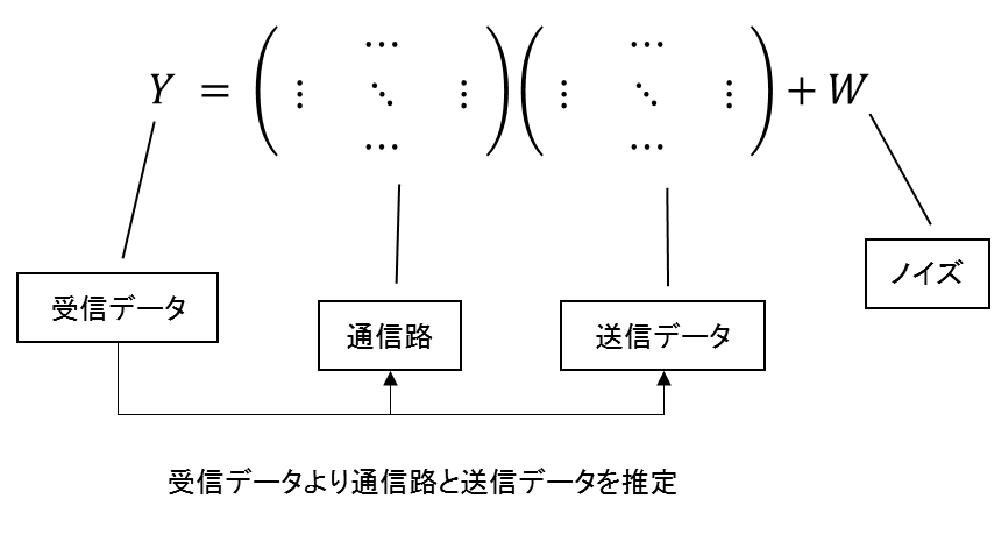
\includegraphics[clip,width=10.0cm]{./matrix.eps}
    \caption{想定しているシステムの行列}
    \label{fig:matrix}
  \end{center}
\end{figure}


\section{論文構成}
\chapter{導出}
\section{近似的確率伝搬法 (Belief Propagetion BP)}
\section{近似的メッセージ伝播法 (Approximate Message Passing AMP)}

\newpage
  \begin{thebibliography}{10}
    \bibitem{soumu_suzuki}
    鈴木 茂樹, ``2020年に向けた情報通信基盤整備の戦略,'', 2014, 2016年11月22日閲覧 \\ {https://www.nic.ad.jp/ja/materials/iw/2014/proceedings/d2/d2-suzuki.pdf}
    \bibitem{suyama}
    須山 聡, シン キユン, 小原 辰徳, 角 誠, 中島 光雅, 奥村 幸彦, ``高周波数帯を用いた超高速MassiveMIMO伝送の基本特性'', 信学技報, 2014年3月.
    \bibitem{goldsmith}
    Abdrea Goldsmith, ``Wireless Communication'', Cambridge University Press, 2005, (訳)小林 岳彦・ 岩切 直彦・大坐畠 智・幸谷 智・高橋 賢・森 香津夫・山嵜 彰一郎, ``ゴールドスミス ワイヤレス通信工学 基礎理論からMIMO,OFDM,アドホックネットワークまで'', 丸善株式会社, , p.297, 2007
    \bibitem{Donoho}
    D. L. Donoho, A. Maleki, and A. Montanari, “Message-passing algorithms for compressed sensing,” Proc. Nat. Acad. Sci. USA, 2009. 
    \bibitem{kabashima}
    Yoshiyuki Kabashima, Florent Krzakala, Marc Mézard, Ayaka Sakata, and Lenka Zdeborová, ``Phase Transitions and Sample Complexity in Bayes-Optimal Matrix Factorization '' , IEEE TRANSACTIONS ON INFORMATION THEORY, VOL. 62, NO. 7, 2016

  \end{thebibliography}
\end{document}

